\subsubsection{MHD: Brio \& Wu Shock Tube}
\label{sec.tests.bw}

A standard test of MHD solvers is the MHD analogue of the Sod shock tube,
described by \citet{Brio88}.   This test, which uses $\gamma=2.0$ and $B_x=0.75$
throughout; $\rho=1.0$, $B_y=1.0$, and $P=1.0$ in the left state; and $\rho=0.125$,
$B_y=-1.0$ and $P=0.1$ in the right state.  A total of 800 grid points were
used, and run to a time of $t=0.08$.  Both tests were run using the HLLD Riemann
solver of \citet{Miyoshi05} and a Piecewise Linear Method \citep{Colella85} reconstruction.  The
results of the test are shown in Figure \ref{fig.brio}.  In that figure, the
black lines show the results of the CT solver while the grey lines show the
reference solution, run at 10,000 points.  A light grey line shows the Dedner
results, but is completely indistinguishable from the points of the CT method.
To highlight the differences between the CT and Dedner solvers, 
the lower pane of each plot shows the difference between the two solutions,
which is at most a few percent.   Most shocks are resolved by a few grid points,
though the contact discontinuity (the large jump seen in density but not
the other quantities) is slightly more smeared.

\begin{figure}
\begin{center}
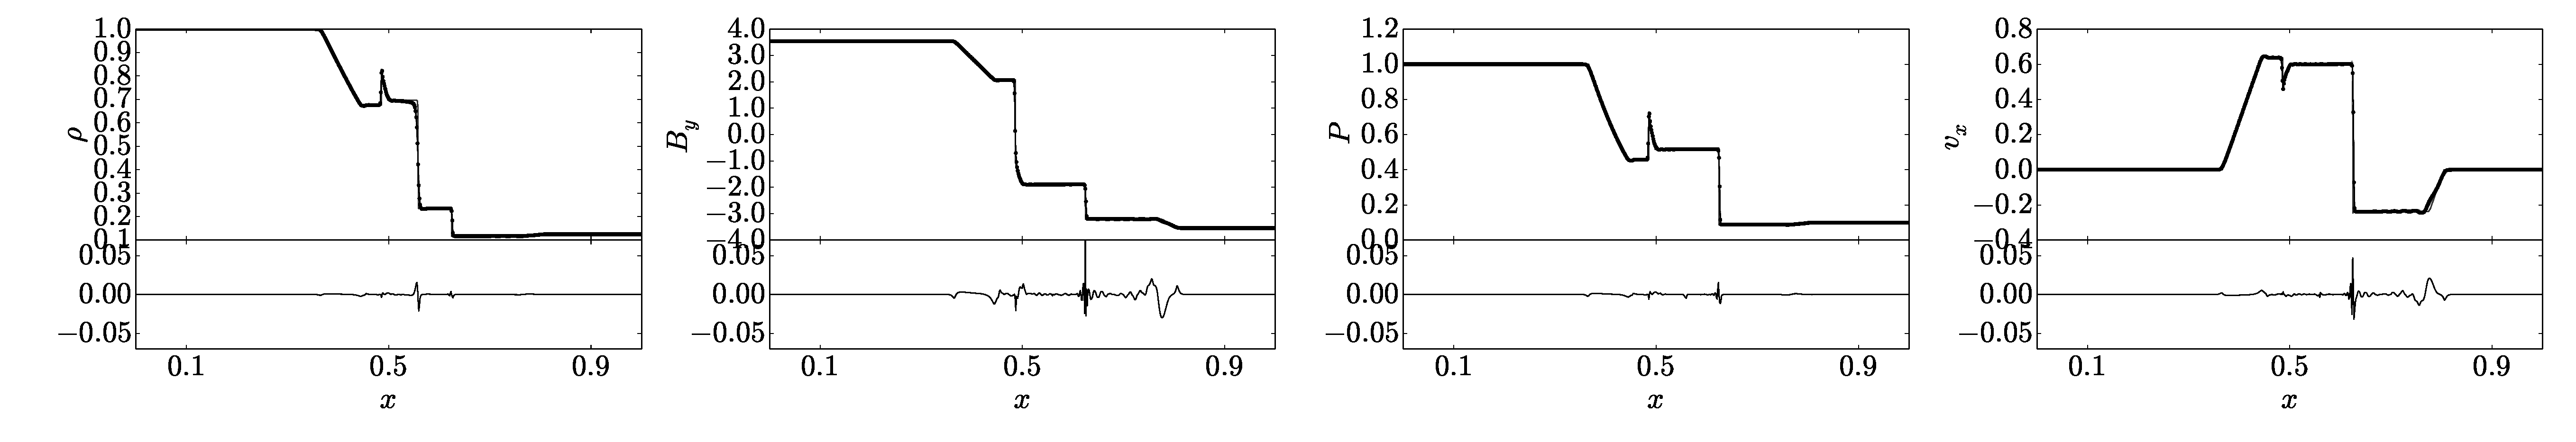
\includegraphics[width=1\textwidth]{figures/bw.eps}
\caption{The shock tube of \citet{Brio88}.  Top panels show the result at
t=0.08
for the CT scheme (black line and points) and Dedner scheme (light grey line,
entirely hidden behind black points) and reference solution, run at 10,000
zones.  Bottom panels
shows the difference between CT and Dedner.}
\label{fig.brio}
\end{center}
\end{figure}
